% Chapter 1

\chapter{Theory} % Chapter title

\label{ch:theory} % For referencing the chapter elsewhere, use \autoref{ch:introduction} 

%----------------------------------------------------------------------------------------

\section{GRASS}

GRASS (Geographical Resources Analysis Support System) is an open source GIS desktop application capable of handling spatial data in both vector and raster formats. 
GRASS adopted a GNU GPL \footnote{General Public License, see http://www.gnu.org} in 1999, which allowed users and developers to have free access to the GRASS source code, resulting in a library of more than 350 freely available modules capable of management, processing, analysis and visualization of geospatial data \citep{GRASSGIS}.\\
Because Open Source GIS provides full access to its internal structure and algorithms, unlike proprietary GIS software, users can learn from existing modules and create their own GIS modules based on the preexisting ones. GRASS libraries can also be accessed through the built-in API (Application Programming Interface). This enables a more efficient integration of new functionalities into the GRASS environment – Most GIS applications can be written in the Python, making it possible to automate work-flows.
As mentioned earlier, GRASS contains around 350 modules, which can be accessed using GRASS' graphic interface. The three main module-groups are based on vector, raster, and imagery analysis \citep{grassbook}.\\

A grass project is located in GRASS' designated database folder \textit{grassdata}(also known as GRASS' GISBASE). This is the directory where processed or imported data is stored and, unless otherwise designated, where most of the processing will occur. 
A project in created in GRASS has to have both a \textsc{LOCATION} and a \textsc{MAPSET}.
The most important of these is the \textsc{LOCATION}. This is where the critical information about the project, such as the projection of the data, is stored. 
GRASS does not have reprojecting on-the-fly functionality – as ArcGIS or QGIS are capable of. Using the \textsc{LOCATION} folder properly is therefore necessary. 
The \textsc{MAPSET} is a way of separating different projects, or phases of processes, and a LOCATION can contain several \textsc{MAPSETS}\citep{grassbook}. 

GRASS can be operated by a variety of ways. The most commonly used method is by accessing the modules through the GRASS GUI (Graphical User Interface), but it can also be achieved purely through scripting – such as with Python. GRASS is able to handle most of the vector and raster formats which are supported by GDAL (Geospatial Data Abstraction Library), such as GeoTIFF, ArcGRID, ERDAS, USGS SDTS DEM, etc \citep{GRASSGIS}.\\

The way GRASS handles region and resolution settings differs from most other GIS software. Since different datasets can have different extents, it is possible to set the current processing region allowing the user to run a specific process on a subset of a raster or the location and not necessarily run a process on the entire image. 
The lack of on-the-fly reprojection makes GRASS less user-friendly than other similar products. Furthermore it does not allow drag and drop import, and most functions must be invoked using the built-in GRASS commandline-like utilities \citep{grassbook}.

\subsection{Hydrology in GIS}

The accurate depiction of hydrological movements and their responses to the land cover has been the objective of hydrological scientists for many decades. As advances in IT have progressed, the calculations and algorithms possible have become more sophisticated, accurate and faster.\\

When investigating hydrological conditions, DEM (Digital Elevation Models) are used. Because of this, the results are dependent on the quality of the model being used. Most major GIS software have some built-in hydrology tools, capable of being incorporated into various workflows. To give an example of the application of hydrology in GRASS, this section will include a description of some of the main hydrology tools from GRASS' libraries.

\subsubsection{Flow direction}
Flow direction is a core hydrology tool. Flow direction makes it possible to determine which direction water will flow, when moving through a DEM. The computational algorithm can be created in a wide variety of ways, for instance GRASS' “r.terraflow” module has two options: 

\begin{itemize}
\item Multiple Flow Direction (MFD) 
\end{itemize}
or 
\begin{itemize}
\item Single Flow Direction (SFD)
\end{itemize}
 
Both of these algorithms are based on a so-called Moore-Neighborhood. This neighborhood involves the eight cells surrounding a specific cell on a raster. The basis of the flow direction is that the water flows to a cell with a lower value then the current one, but it is in this regard that MFD and SFD differ from each other. As can be seen from \autoref{fig:flowdirect}, the SFD method assigns a single flow direction to the lowest downslope neighboring cell, whilst MFD assigns flow direction to all downslope neighboring cells \citep{grassbook}. \\
\begin{figure}[t]
\centering
	{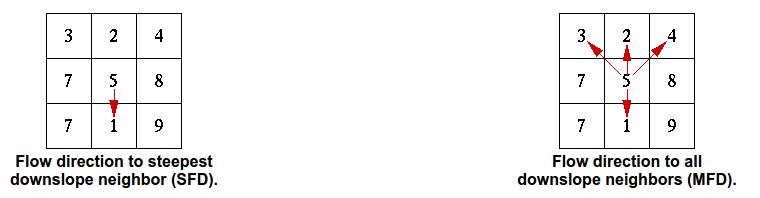
\includegraphics[width=\linewidth]{gfx/SFD_MFD.png}}
\caption{Example of two different flow direction methods \citep{sfdmfd}.}
\label{fig:flowdirect}
\end{figure}
Both methods have the criteria, that the flow direction cannot contribute to cells with the same height as the central cell or cells which have no downslope neighbors \citep{sfdmfd2}.
Pits or so called depressions or sinks, are areas which are surrounded by higher elevation values. It is also an internal drainage area, although some of the time it is a real natural feature such as a karst, but usually it is an imperfection of the digital elevation model.  The GRASS Terraflow module fills the sinks and then assign a Flow Direction on the filled terrain, thereby the flow direction will not be ruined by a DEM full of depressions \citep{sfdmfd}. 

\subsubsection{Flow accumulation}
Another important hydrology tool is Flow Accumulation. This tool is capable of calculating the flow running through the the terrain, such as the accumulation of water \citep{sfdmfd}. As input, the module needs a raster indicating flow directions. \\ 
It should be noted that flow accumulation is highly dependent on the previous described phenomenas and computational methods. For example MFD would provide a significantly different flow accumulation than SFD, as MFD provides more accumulation possibilities. Also, a depressionless DEM will have a different accumulation than one with depressions \citep{sfdmfd}. Analyzing the direction of the flow can give a limited insight about cell behaviors, however flow accumulation allows the investigation of main stream lines, and how they contribute to the stream system, as well as providing the an output of stream lines.

\subsubsection{Watershed}
A Watershed is an area where all streams end up in a common outlet. This can also be called a basin or a catchment area, however in this paper it will be referred to as a watershed.\\


\begin{figure}[h]
\centering
	{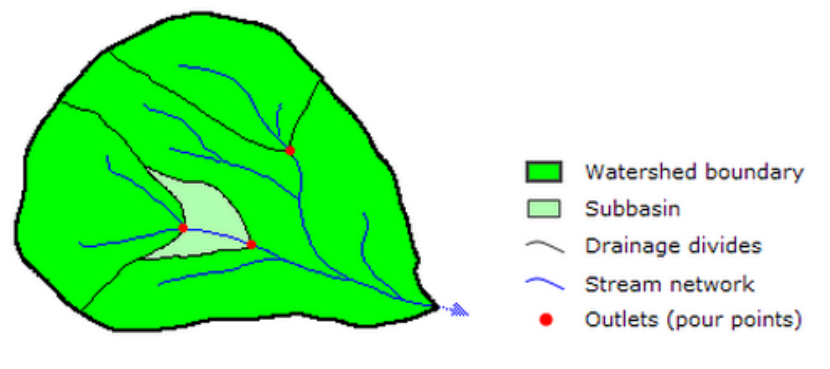
\includegraphics[width=\linewidth]{gfx/Watershed.png}}
\caption{Figure showing important concepts when working with watersheds \citep{watershed}.}
\end{figure}

A watershed is a relative term, as it depends on the scale at which you look at them – practically all streams have their own watershed. Therefore to determine the watersheds of a DEM, it is necessary to know a variety of factors, such as flow accumulation, flow direction or slope aspect of the terrain \citep{rwatershed}.\\

In  GRASS there is a watershed algorithm, which considers every aspect of the previously mentioned procedure. The watershed (r.watershed) module has watershed output which is created by the output of the flow direction and the derived flow accumulation output of the DEM. As mentioned earlier, watershed sizes are relative to the scale of the investigation. A threshold value can be set the to delineate the minimum size of the resultant watershed, based on the scale of interest \citep{grassbook} \citep{rwatershed}. Setting this value should be based on the horizontal resolution of the raster being worked on. For instance, setting the value to 1000 setup on a raster with 10mx10m resolution, would define, that the smallest watershed area has to be larger than 1000*10m*10m = 0,1km2.

\subsubsection{Cost Distance}
The Cost Distance analysis is used to calculate the route that will “cost” the least when traveling across a given surface \citep{grassbook}. This tool uses a cost surface to determine the weighted shortest path to the nearest source cells or source vector feature, and as such does not calculate distance in geographical units, but shows the distance by cost surface units \citep{rcost}. The cost can include several criteria, factors and weights depending on the specific analysis. For example, the cost surface of a hiking route can be established by taking into account the steepness, the type of the area or even the recommendations of which area should be visited.\\
Each of the factors chosen should be reclassified in order to put them on a common scale, so that they can be compared in spite of their different nature. 
The cost distance module of GRASS (r.cost) is based on the previously explained method \citep{rcost}. In order to get the cost distance output raster, the user needs to provide a cost raster.

\begin{figure}[t]
\centering
	{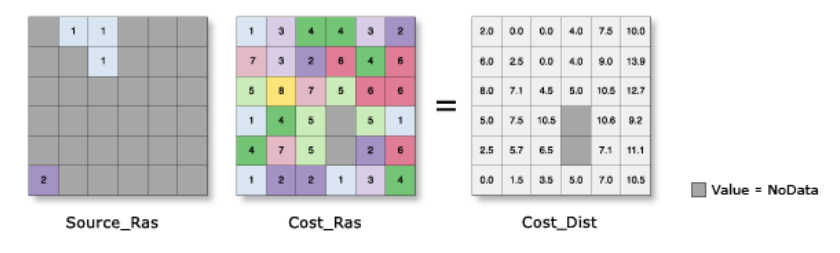
\includegraphics[width=\linewidth]{gfx/COST.png}}
\caption{Figure showing how cost distance works \citep{costdistance}.}
\end{figure}

%----------------------------------------------------------------------------------------

\section{Python}\label{sec:issues}

Python is a programming language used extensively within the geospatial world. A lot of GIS packages are either created with Python, or have built-in functionality to inferface with Python. The actual reason for this is generally not known, but it might be because Python is a language that \citep{pybook}:
\begin{itemize}
\item emphasizes code readability.
\item is compatible with all major operating systems, and usually comes pre-packaged with these. 
\item Is completely open source. 
\item is highly extensible. 
\end{itemize}
Being extensible, means that it does not come prepackaged with all functionality built in, but expects the user to download / add necessary libraries as they are needed. 
The most commonly used versions of Python are 2.7 and 3.x, which differ from each other for various reasons. The 2.7 release is a so-called legacy release, which means that it is not the worked-upon version, and wont see major updates. The 3.x is the newest version, and will be updated regularly. When working with “older” software, and libraries, it is most likely best to use version 2.7 as there will likely be compatibility issues when using a newer version of Python \citep{python}.\\

Standard python syntax looks something like this:\\

\begin{lstlisting}[language=Python]
import random
randomarray = [1,3,5,7,8]
for element in randomarray:
	print(element)
\end{lstlisting}

\section{GRASS}

From within GRASS, Python can easily be used to call native functionality. These functions can also be accessed and manipulated by using a variety of scripting languages, without explicitly starting the GRASS software. One of the languages capable of doing this is Python. \citep{grassbook} \\

Opening, and chaining, functions within GRASS can become tedious, and if wanting to run the same process a lot of times, it can be relevant to setup a workflow with a Python script.
The functions and modules of GRASS, when used outside of an actual GRASS session, only work when a series of specific environment variables have been set. 
These are \citep{grasswiki}:
\begin{itemize}
\item GISBASE needs to be set to the top-level directory of the GRASS installation. 
\item GISRC needs to contain the absolute path to a file containing settings for GISDBASE, LOCATION and MAPSET 
\item PATH needs to include \$GISBASE/bin and \$GISBASE/scripts.
\end{itemize}

An example of the syntax of GRASS functions being accessed externally through Python \citep{grasswiki}:

\begin{lstlisting}[language=Python]
import grass.script as gscript
import grass.script.setup as gsetup
gscript.run_command(“r.in.gdal”,flags=””,input=”input.tif”,output=”output”
\end{lstlisting}


\section{Web technologies}
\subsection{HTML}
In 1990, Tim Berners-Lee, a physicist employed at CERN, invented HTML by trying to organize the research documents available to scientists and facilitate their access to them. He is also considered by many the inventor of the Internet by having set the foundations of the web as we know it today \citep{htmlnet}.
HTML stands for HyperText Markup Language. To be more specific \citep{htmlnet},

\begin{itemize}
\item Hyper means that HTML does not perform commands in one line and then proceeds to the next one as Python or C++ does.
\item Text is self-explanatory
\item Markup means that the author can put tags in the text. This means that the text is structured in different sections such as the header, the body etc.
\item Language of course means that HTML is a programming language.
\end{itemize}

The following figure displays an example of a basic HTML code snippet. It will help in understanding the structure and content of an HTML document.

\begin{lstlisting}
<!DOCTYPE html>
<html>
<body>

<h1>My first heading!</h1>
<p>My first paragraph!</p>

</body>
</html>
\end{lstlisting}

Starting at the top, the DOCTYPE declaration, states what kind of document we are creating. In this case, we have an HTML document (w3shcools). In the html tags (<html>, </html>), we describe the page we are creating. The body tags (<body>, </body>) contains all the information visible to the user. Finally, the tags <h1> and <p>, set the heading and paragraphs respectively \citep{w3schools}.

\subsection{JavaScript}
JavaScript is a dynamic scripting language developed by Netscape. Brendan Eich, the original developer of JavaScript, created it so that it would be able to support prototype based object construction and  that it can work both as an object oriented and procedural language. Its syntax was developed to be similar to C++ and Java in order to minimize its learning curve \citep{mozjava}. Below, we can see a small example of JavaScript use in an HTML document.	

\begin{lstlisting}
<!DOCTYPE html>
<html>
<body>

<h1>My first JavaScript!	</h1>

<script>
document.write("<p>My First Javascript!</p>");
</script>

</body>
</html>
\end{lstlisting}

In this example, we have a basic HTML document and in the script tags (<script>, </script>) we can insert the JavaScript function that will be executed.

\section{PyWPS}

A Web Processing Service (WPS) is a standard defined by the Open Geospatial Consortium which describes how inputs and outputs (also called requests and responses) for geospatial processing services should be standardized. 
WPS Version 1.0 was released in June 2007, and WPS version version 2.0 was approved and released in January 2015 \citep{ogcwps}. \\
WPS defines how a client can request the a process is executed, and how the output is supposed to be handled. Furthermore, it defines the setup of the interface that enables publishing of geospatial processes, and the user's access to those processes. Through this implementation, it should become easier for people who want to publish custom geospatial functions on the internet, to do it in a similar and organized way. \\

One implementation of these standards is PyWPS. This service connects the web browser with a variety of tools installed on a server, such as GRASS GIS, GDAL, PROJ and R \citep{pywpsweb}. PyWPS does not process the data by it self but  it can work with GIS software such as GRASS, enabling the creation of GIS-based analytical web services, based on Python \citep{pywpsweb}. 
The WPS enables a user to Describe a Process, Execute a Process and to Get Capabilities of the server, and the instances available. Similar to other OGC Web Services (such as WMS, WFS or WCS), WPS has three basic request types. Namely GetCapabilities, DescribeProcess and Execute \citep{pywps}.\\

When requesting data from the server, the URL you send to the server, defines what kind of request you have made. Example strings for the three processes mentioned above:\\
\begin{itemize}
\item http://webaddress/pywps/?service=WPS&request=GetCapablities 
\item http://webaddress/pywps/?service=WPS&version=1.0.0&request=DescribeProcess&identifier=all
\item http://webaddress/pywps/?service=WPS&version=1.0.0&request=Execute&identifier=<PROCESS>&datainputs=[<INPUT1>=<VALUE>;<INPUT2>=<VALUE>]
\end{itemize}

When an Execute request has been posted to the WPS, it will start processing on the server, and when it is done outputs will be provided encoded in a standardized XML document. 
A PyWPS service must contain the following elements \citep{pywps}: 
\begin{itemize}
\item A class defining the initation of a WPS Process:
class Flooding(WPSProcess):
\item A function called \_\_init\_\_:
def \_\_init\_\_(self):
\item A function called execute:
def execute(self):
\end{itemize} \\

The init function contains a variety of settings relevant to the process being executed. Furthermore the inputs and outputs get defined, whilst the execute contains the code that is to be run. 
The PyWPS syntax for calling GRASS differs somewhat from when interfacing purely with Python. An example of GRASS accessed with PyWPS is:

\begin{lstlisting}[language=Python]
self.cmd(['r.in.gdal','input=%s' % self.rasterin.getValue(),'output=%s' % original,'-o'])
\end{lstlisting}

\section{Flask}

Flask is a web application framework written in Python. The framework is based on a so-called Web Server Gateway Interface (WSGI) called Werkzeug and a website templating engine called Jinja2. The framework is built to be as simple as possible, comes with a core of the most needed libraries, and expects further functionalities and modules to be imported as third-party libraries \citep{flaskbook}. \\
Several similar frameworks exist, but they either become very advanced, or very specialized. The Flask framework has a simple setup, and is easy to use. \citep{flaskbook} \\
By using Flask it is possible to quickly create a dynamic web environment, by writing it in a combination of Python and HTML. 
A simple application using Flask looks something like the following \citep{flaskweb}: 

\begin{lstlisting}[language=Python]
from flask import Flask
app = Flask(__name__)

@app.route("/")
def hello():
    return "Hello World!"

if __name__ == "__main__":
    app.run()
\end{lstlisting}

A website written in Flask consists of a variety of templates that change content depending on where on a site a user is, or wishes to visit. This is done by defining some general templates, and some blocks of content that get swapped out depending on the current view. 

%----------------------------------------------------------------------------------------

\section{Open Source GIS}

The definition of Open Source is clearly set by the Open Source Initiative (OSI), making it possible to clearly define define which licenses actually are "Open Source". In addition to this, the OSI provides certification to these licenses to indicate that they follow the open-source principles and comply with the Open Source definition. This definition states the following \citep{osbook}:
\begin{itemize}
\item The license should allow the sale or gifting of the software as a part of software distribution along with programs from several different sources. For such sale no royalty or monetary compensation should be required. ("The license shall not restrict any party from selling or giving away the software as a component of an aggregate software distribution containing programs from several different sources. The license shall not require a royalty or other fee for such sale".)
\item The source code of the software should be included in the software and it must be distributed freely along with the compiled form. In the case where the source code is not distributed with the software, an easily reached alternative must be provided, at most with a minimum reproduction cost.
\item Modifications and derived works must be allowed and distributes as freely as the software itself.
\item Modification of the source code can be restricted by the license only in the case that the license allows "patch files" distribution along with the source code for program modification. Software built from modified source code must be allowed to be distributed. 

\begin{figure}[H]
\centering
	{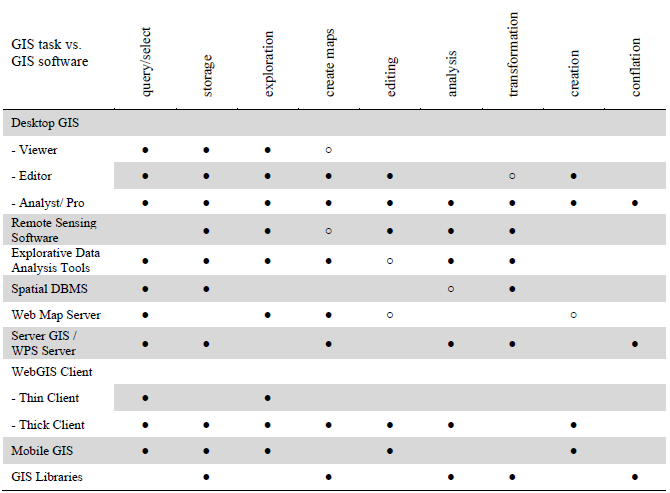
\includegraphics[width=\linewidth]{gfx/OS.png}}
\caption{Figure showing categorization of GIS software \citep{osarticle}}
\label{fig:giscategory}
\end{figure}

\item Works derived from the source code may be required to have a different name or version number.
\item Discrimination against persons or groups is not allowed
\item All fields of endeavor must be allowed to use the software, unrestricted by its license. In the case where the program is redistributed, the same rights must apply without the execution of an additional license from those parties.
\item In the case where the program is part of a specific software distribution, parties to whom the program is redistributed should have the same rights with those to  whom the original program is distributed.
\item Restrictions on other software, distributed with the licensed software must not be placed under restrictions.
\item Access to the license must not be dependable on any individual technology pr interface
\end{itemize}

Some of the most common desktop GIS Software can be seen from \autoref{fig:giscategory}.
The main reason open software exists is because the US Government, during the 1970ies and 1980ies implemented changes in the patent laws that allowed software and hardware companies to unbundle software and hardware and the source code for software was under restricted access. For the reasons stated above the Free Software Foundation (FSF) was created \citep{osbookde}.

\begin{table}[H]
\caption{GIS software}
\begin{tabular}{ l | p{0.55\linewidth} }
Desktop GIS Software & Developer \\ 
\hline
GRASS GIS & Neteler \& Mitasova, 2008 \newline
Neteler, Bowman, Landa \& Metz 2012 \\ 
\hline
QGIS & Hugentobler, 2008 \\ 
\hline
ILWIS / ILWIS Open & Valenzuela, 1988 \newline
Hengl, Gruber \& Shrestha, 2003 \\ 
\hline
uDig & Ramsey, 2006 \\ 
\hline
SAGA & Olaya 2004, Conrad 2007  \\ 
\hline
OpenJUMP & Steiniger \& Michaud, 2009 \\ 
\hline
MapWindow GIS & Ames, Michaelis \& Dunsford, 2007 \\ 
\hline
gvSIG & Anguix \& Diaz, 2008 \\ 
\hline
\end{tabular}
\caption*{Categorization of GIS software \citep{osarticle}.}
\label{tab:gissoftware}
\end{table}

Due to their widespread need, Geographic Information Systems software are also available to the public under the "Open Source" label. These software include a wide variety of open source examples that can be divided based on the functionalities the offer. \autoref{tab:gissoftware} below can provide with some insight on such categorization. 

\section{Digital Elevation Models}
A Digital Elevation Model (DEM) is a collection of three-dimensional points (X, Y, Z)that describe the Earth's ground elevation. Often stored in raster format, these models hold a very important role in the fields of photogrammetry, remote sensing and mapping. They also are a valuable component in the process of orthophoto creation along with aerial and satellite imagery. There are many ways someone can create a DEM \citep{dem}:

\begin{enumerate}
\item From surveying and topographic maps
\item Using aerial imagery
\item From LiDAR data
\item Through satellite imagery
\end{enumerate}

Apart from the DEM, other elevation models can be created, using the same methods, that describe other aspects of the Earth's surface. One of the most widely used models is the Digital Surface Model (DSM). In this Elevation Model, the points that comprise it, describe the surface of the Earth and all the elements on it, either man-made or natural.

\paragraph{Danish Elevation Models:} The Danish elevation models (DK-DEM) are created using LiDAR point clouds. The latest fully available elevation models and LiDAR point clouds were collected from 2005 to 2007, by two Danish companies (Blominfo and Scankort A/S). Responsible for the quality control of the elevation models was the Danish National Survey (KMS). The DK-DEM is using UTM32N/ETRS89 as horizontal reference system and DVR90 as vertical reference \citep{demdk}.
In order to estimate the accuracy both vertical and horizontal, a number of control measurements were performed using sophisticated GPS instruments. As far as the vertical accuracy is concerned, the average Root Mean Square (RMS) error was 5.9cm while the standard error was 3.44cm. As far as the horizontal accuracy is concerned, the process in order to calculate it included using 568 corners of 142 buildings. The results from this process resulted in an average RMS error of 67cm \citep{demdk}.

